\usetikzlibrary{shapes.geometric}
\usetikzlibrary{positioning}

\newcommand{\apparatus}[4]{\node[square node] (#1) at (#2,#3){#4};
                           \node[port] (#1+) at (#2 + 0.375, #3 + 0.5){+};
                           \node[port] (#1-) at (#2 + 0.375, #3 - 0.5){-};}

\chapter{Stern-Gerlach Experiments}

TODO: provide a brief explanation of the experimental setup and results. Discuss historical and pedagogical significance. Explain how measurement results correspond to the particle's localization in certain regions. This section is background information so that I can discuss the von Neumann measurement, consistent histories, and decoherence in the context of this experiment. I am saving it for later to focus on the introducing the new theory for now.

\chapter{Postulates of Quantum Mechanics}

We first consider the mathematical objects used to model physical systems and variables. By comparing the objects used in classical and quantum mechanics, we make sense of the first three postulates of quantum mechanics. Then, we compare the Copenhagen and von Neumann descriptions of measurement and their relation to the fourth and fifth postulates.

\section{Physical Variables and State Spaces}
\subsection{Classical States}
Consider the spin of an electron. Treating the electron as a classical system, its spin state is modeled by a vector $\vec{S} \in \mathbb{R}^3$:
\begin{align}
\vec{S} = (S_x, S_y, S_z)
\end{align}

Each component $S_{x_i}$ is a physical variable representing the magnitude of spin oriented in the $\hat{x_i}$ direction.

$\vec{S}$ has the capacity to determine spin in any direction using the inner product of the state space $\mathbb{R}^3$:
\begin{align}
S_n(S) = \vec{S} \cdot \hat{n}
\end{align}

We see that in classical mechanics, physical variables are modeled using functions. Each function $S_n$ maps a spin state $[\vec{S}$ to a real scalar representing the spin of the electron aligned along the $\hat{n}$ axis.

What makes classial mechanics more familiar to everyday experience boils down to intuitive but important properties of the state space $\mathbb{R}^3$:
\begin{itemize}
\item For any direction $\hat{n}$, $\vec{S}$ determines spin $S_n$
\item $S_n$ can be any real value
\end{itemize}

$\vec{S}$ determines spin in any direction because TODO. Consequently, the sample spaces for spin in any two directions $\hat{n}$ and $\hat{m}$ are \textit{compatible}, meaning that $S_n$ and $S_m$ may be simultaneously determined. Spin states in $\mathbb{R}^3$ are interpreted physically as the electron posessing definite values for every $S_n$ at some instant in time.

In addition to spin states determing all $S_n$, the state space allows $S_n$ to take on any real value. There are no fundamental restrictions on which real numbers $S_n$ could be; its sample space is continuous and infinitely large.

\subsection{Quantum States}
Measurements of electron spin show that the intuitive classical properties do not hold. Recall that only two magnitudes of spin have ever been measured. $S_n$ is a \textit{quantized} physical variable; its sample space is discrete and finite.

Second, the results of successive measurements of a spin system imply that $\vec{S}$ does not determine spin in some general direction $S_n$. Recall the results of succesively measuring spin in orthogonal directions discussed in (TODO ref). After measuring $S_x$, $\vec{S}$ appears to ``forget'' a previous measurement of $S_z$. All we may know about the system at one instant in time is spin in one direction. The inabilitiy to simultaneously determine spin in two independent directions $\hat{n}$, $\hat{m}$ should be reflected through $S_n$ and $S_m$ having \textit{incompatible} sample spaces.

Electron spin measurements violate the intuitive classical state space properties mentioned in 3.1.1. In response, we must change the mathematical objects used to represent system states and physical variables. Specifically, the sample space of $S_n$ must restrict observable values to spin up and spin down, and $S_n$ and $S_m$ should have incompatible sample spaces. In combination, the first three postulates of quantum mechanics takes care of these differences.

Quantum mechanics postulates that a system state is completely described by a normalized vector in a linear state space.

\invisiblesubsubsection{Postulate 1 (System States)}
\begin{Thm:Postulate}{1}
    The state of a physical system is defined by specifying an abstract vector $\ket{\psi}$ in a Hilbert state space $\mathcal{H}$.
\end{Thm:Postulate}

For spin-$\frac{1}{2}$ systems such as electrons, the two-dimensional Hilbert space consists of all linear combinations of spin-up and spin-down:
\begin{equation}
    \mathcal{H} = \{\alpha\ket{+} + \beta\ket{-}\}
\end{equation}
where $\alpha, \beta \in \mathbb{C}$.

$\mathcal{H}$ is an abstract state space; components of $\ket{\psi}$ cannot be interpreted as physical variables as they are for the classical spin state $S$. So, we introduce physical meaning with more postulates.

\invisiblesubsubsection{Postulate 2 (Physical Variables as Operators)}
The second posulate of quantum mechanics states that physical variables are described by linear operators:
\begin{Thm:Postulate}{2}
    Every physical variable $\mathcal{A}$ is described by an operator $A$ acting in $\mathcal{H}$.
\end{Thm:Postulate}

\invisiblesubsubsection{Postulate 3 (Observable Values)}
Justifying the second postulate is easiest when also considering the third postulate:
\begin{Thm:Postulate}{3}
    The only possible result of the measurement of a physical variable $\mathcal{A}$ is one of the eigenvalues of the corresponding operator $A$.
\end{Thm:Postulate}

The operator correlates elements of a finite sample space (eigenvalues) with particular system states (eigenstates). Consequently, a state can only be interpreted as having a definite variable value if it is an eigenstate of that variable's operator. To illustrate this, consider the operator representing $S_z$. Written in the basis of its own eigenstates,
\begin{align}
    S_z \doteq \frac{\hbar}{2}\begin{bmatrix} 1 & 0 \\ 0 & -1 \end{bmatrix}
\end{align}
This operator correlates $z$ spin-up $\left(S_z = \frac{\hbar}{2}\right)$ with eigenstate
\begin{align}
    \ket{\psi} = \ket{+}_z \doteq \begin{bmatrix} 1 \\ 0 \end{bmatrix}
\end{align}
and $z$ spin-down $\left(S_z = \frac{-\hbar}{2}\right)$ with eigenstate
\begin{align}
    \ket{\psi} = \ket{-}_z \doteq \begin{bmatrix} 0 \\ 1 \end{bmatrix}
\end{align}
Similarly, the operator representing $S_y$ written in the $S_z$ basis is
\begin{align}
        S_y \doteq \frac{\hbar}{2}\begin{bmatrix} 0 & -i \\ i & 0 \end{bmatrix}
\end{align}
This operator correlates $y$ spin-up $\left(S_y = \frac{\hbar}{2}\right)$ with eigenstate
\begin{align}
    \ket{\psi} = \ket{+}_y \doteq \frac{1}{\sqrt{2}}\begin{bmatrix} 1 \\ i \end{bmatrix}
\end{align}
and $y$ spin-down $\left(S_y = \frac{-\hbar}{2}\right)$ with eigenstate
\begin{align}
    \ket{\psi} = \ket{-}_y \doteq \frac{1}{\sqrt{2}}\begin{bmatrix} 1 \\ -i \end{bmatrix}
\end{align}

Operators for $S_z$ and $S_y$ share no common eigenstates, so no state can posses definite values for both variables. In general, operators for any two spin components $S_i$ and $S_j$ do not share common eigenstates with each other; in other words, $S_i$ and $S_j$ have incompatible sample spaces.

By representing physical variables with operators rather than functions, sample spaces become quantized and may be incompatible with each other. These features are necessary for predicting the results of electron spin measurements.

The first three postulates designate the mathematical objects used to model physical system states and variables. The fundamental differences between classical and quantum systems are completely described by these postulates and their consequences.

\subsection{Linearity}
TODO: compare addition of $S_x, S_y$ states and their interpretations. Introduce superposition states and coherence.

\section{Copenhagen Description of Measurement}
The fourth and fifth postulates constitute the Copenhagen description of measurement. This description is a key component of the standard interpretation of quantum mechanics, taught in textbooks and introductory quantum courses worldwide.

The probability postulate, also known as the \textit{Born Rule}, assigns a probability distribution to the sample space of a physical variable.

\invisiblesubsection{Postulate 4 (Probability Distribution of Measurement Outcomes)}
The second posulate of quantum mechanics states that physical variables are described by linear operators:
\begin{Thm:Postulate}{4}
    When measuring physical variable $A$, the probability $\mathcal{P}(n)$ of obtaining result $a_n$ corresponding to $\ket{a_n}$  is equal to
     \begin{align}
        \mathcal{P}(n) = |\braket{_na|\psi}|^2
    \end{align}
\end{Thm:Postulate}

The probabilities assigned to each state leaving the $S_x$ Stern-Gerlach device in Figure \fref{Figure:Measurement:DetectorStates} are
\begin{align}
    \mathcal{P}_{+_y} &= |_y\braket{+|+}|^2 = \frac{1}{2} \\
    \mathcal{P}_{-_y} &= |_y\braket{-|+}|^2 = \frac{1}{2}
\end{align}

The spirit of the Born Rule is unchanged in consistent quantum theory. Differences are discussed in (TODO: ref future section).

\invisiblesubsection{Postulate 5 (Collapse Dynamics)}

The fifth postualte (known as the projection postulate) describes how a system evolves upon measurement. Contingent upon interaction of the system with a ``classical apparatus'', measurement instantaneously changes the state of the system to the eigenstate corresponding to the measurement result.

\begin{Thm:Postulate}{5}
    If the measurement of the physical variable $\mathcal{A}$ on the system in the state $\ket{\psi}$ gives the result $a_n$, the state of the system immediately after the measurement is the normalized projection
    \begin{align}
        \ket{\psi}^\prime = \frac{P_n\ket{\psi}}{\sqrt{\bra{\psi}P_n\ket{\psi}
        }}
    \end{align}
    onto the subspace associated with $a_n$.
\end{Thm:Postulate}

${P^n}_z = \ket{n}_z\tensor[_z]{\bra{n}}{}$ is the projection operator for the state $\ket{n}_z$ corresponding to $n_z$.

Consider a measurement result for the $z$ component of spin, $S_z$. We represent the result with $n_z$, which could be either spin-up or spin-down. The new state is the normalized projection of $\ket{\psi}$ onto $\ket{n}_z$. In other words, $\ket{\psi}$ instantaneously becomes $\ket{n}_z$ upon measurement. This process is known as \textit{state collapse} or \textit{wavefunction collapse}.

\begin{figure}
\centering\CaptionFontSize
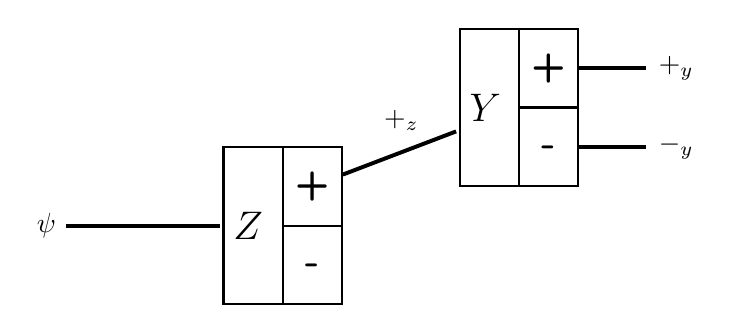
\begin{tikzpicture}[shorten >=1pt,auto, thick,
     square node/.style={rectangle, minimum height=2cm, minimum width=1.50cm, text width = 1.25cm, draw, font=\sffamily\Large\bfseries},
     port/.style={rectangle, draw,  minimum height=1cm, minimum width=0.75cm, font=\sffamily\Large\bfseries},
     wf/.style={rectangle, minimum height=1cm}]
    \apparatus{1}{3}{0}{$Z$};
    \apparatus{2}{6}{1.5}{$Y$};

    \node[wf] (w0) at (0,0) {$\ket{\psi}$};
    \node[wf] (w1) at (8, 2.0) {$\ket{+}_y$};
    \node[wf] (w2) at (8, 1.0) {$\ket{-}_y$};

    \draw[line width=0.5mm] (w0) -- (1);

    \draw[line width=0.5mm] (1+) -- (2) node [near end] {$\ket{+}_z$};

    \draw[line width=0.5mm] (2+) -- (w1);
    \draw[line width=0.5mm] (2-) -- (w2);
\end{tikzpicture}
\caption[Insert an abbreviated caption here to show in the List of Figures]
{The Stern-Gerlach experiment as described by the standard measurement scheme. Notice that each measurement
outcome is renormalized, so that information about the state prior to measurement is lost.}
\label{Figure:Measurement:Renormalizing}
\end{figure}

As an example, consider the system shown in \fref{Figure:Measurement:Renormalizing}. The first apparatus serves as a state preparation device, since we are only interested in particles exiting the spin-up output. Using the projection postulate, the state after the first measurement is
\begin{align}
    \ket{\psi_{top}} &= \frac{{P^z}_+\ket{\psi}}{\sqrt{\bra{\psi}{P^z}_+\ket{\psi}}} = \ket{+}_z
\end{align}
Similarly, the possible output states from the second apparatus are
\begin{align}
    \ket{\psi_{top}} &= \frac{{P^y}_+\ket{+}_z}{\sqrt{\tensor[_z]{\bra{+}}{}{P^y}_+\ket{+}_z}} = \ket{+}_y \\ \\
    \ket{\psi_{bottom}} &= \frac{{P^y}_-\ket{+}_z}{\sqrt{\tensor[_z]{\bra{+}}{}{P^y}_-\ket{+}_z}} = \ket{-}_y
\end{align}

TODO: carry out example calculations using Born rule

\section{Dynamics}
\invisiblesubsubsection{Postulate 6 (Unitary Dynamics)}
TODO: introduce 6th postulate (Schrodinger time evolution)

\chapter{Measurement}

TODO: chapter preview

\section{Issues with State Collapse}
In a mechanical theory, the equations of motion (or \textit{dynamics}) describe how a state evolves with time. In classical Newtonian mechanics, this is given by Newton's law of motion
\begin{align}
  \vec{F} = m\vec{a}.
\end{align}

These dynamics are \textit{unitary}, meaning that given the final state of a physical process, the corresponding initial state is recovered by applying the dynamics with time reversed. The dynamics can be represented by a one-to-one map from initial to final states.

Standard quantum mechanics postulates two separate types of dynamics. The unitary dynamics described by the Schrödinger equation are analogous to Netwon's law of motion. In contrast, the non-unitary dynamics described by the projection postulate have no classical analog. When applied, all information about the initial state is lost as the state instantaneously becomes an eigenstate of the measured variable. The map from initial to final states is not one-to-one.

TODO: interpretational issues

Because the measurement process cannot be reversed, state collapse injects time asymmetry into the foundations of quantum mechanics. TODO: discuss arrow of time.

In addition to the red flags that come with non-unitary dynamics, the projection postulate relies on ambiguous definitions. State collapse occurs upon ``interaction with a classical measuring apparatus'', yet there is no specification of what makes a system classical. Classical systems are not described by the theory, yet they play a fundamental role in the measurement process.

The issues with interpretation of state collapse and non-unitary dynamics in general are indicators that collapse dynamics are formulated with ignorance of some underlying process. To begin describing this process, we seek to discard the projection postulate and describe measurement using dynamics permitted by the Schrödinger equation.

Describing measurement as a unitary process is desirable for multiple reasons:
\begin{itemize}
  \item With dynamics symmetric in time, the emergence of the ``arrow of time'' can be studied
  \item Humans and measurement apparatuses do not play a special role indescribale by the theory
  \item TODO: describe cosmology benefit.
  \item interpretational issues with state collapse go away
  \item less fundamental assumptions
\end{itemize}

Fortunately, such a description is possible using the von Neumann measurement scheme.

\section{von Neumann Measurement Scheme}
In the discussion of Stern-Gerlach experiments, the position of the electron has played an implicit role in measurement. In exemplifying use of the TODO REF projection posulate, we define a measurement result as the localization of the electron in the spin-up or spin-down regions. The primary measurement is that of position, which is used to imply the spin state, yet the position system is never formalized.

Our goal is to use the von Neumann measurement scheme to formalize the correlation of position and spin eigenstates we observe in Stern-Gerlach experiments. We start by representing the electron with a composite spin-position system,
\begin{align}
  \mathcal{H} = \mathcal{H}_s \otimes \mathcal{H}_x
\end{align}

\subsection{Example 1}
We revisit the example of one Stern-Gerlach measurement of spin along the $z$ axis. To simplify calculations, we define coarse grainings of position states. $\ket{+_x}$ and $\ket{-_x}$ represent localization within the spin-up and spin-down regions, respectively. We also group all other position eigenstates, representing it with $\ket{\varnothing_x}$; this is the position of an electron not being measured by the apparatus. The states $\{\ket{+_x}, \ket{-_x}, \ket{\varnothing_x}\}$ form an orthogonal and exhaustive basis for the position space. TODO: also assert normality? Figure.

We introduce an operator that correlates these position states with spin eigenstates in explicit form:
\begin{align}
  U(t_0, t_1) &= P^z_+ \otimes \left(\: \ket{+_x}\bra{\varnothing_x} \: \bm{+} \: \ket{\varnothing_x}\bra{+_x} \: \bm{+} \: \ket{-_x}\bra{-_x} \: \right) \\ \nonumber
  &+ P^z_- \otimes \left( \: \ket{-_x}\bra{\varnothing_x} \: \bm{+} \: \ket{\varnothing_x}\bra{-_x} \: \bm{+} \: \ket{+_x}\bra{+_x} \: \right)
\end{align}

Starting with a general spin state, the final state is
\begin{align}
  U(t_1, t_0)\ket{\psi} & =  U(t_1, t_0) \left(\ket{\psi_s} \otimes \ket{\varnothing_x} \right) \\
  &= \nonumber P^z_+ \ket{\psi_s} \otimes \ket{+_x} \: \bm{+} \: P^z_- \ket{\psi_s} \otimes \ket{-_x}
\end{align}

At the instant measurement begins $t_0$, the position state is $\ket{\varnothing_x}$ as the electron enters the magnetic field. At the instant measurement ends $t_1$, the position state is either $\ket{+_x}$ or $\ket{-_x}$, realized with spin-up and spin-down spin states respectively. Notice that the final sum does not contain any terms representing incorrect correlations between spin and position states (such as $ P^z_+ \ket{\psi_s} \otimes \ket{-_x}$).  Consequently, the final state cannot be written as the tensor product of a state in $\mathcal{H}_s$ and a state in $\mathcal{H}_x$ (as the inital state was). This is the definition of \textit{entanglement}; the von Neumann measurement scheme describes the measurement process as entanglement.

The von Neumann scheme is usually written as a linear map:
\begin{align}
    \nonumber U(t_1, t_0): \\
    & \ket{\psi} = \left(\sum_{n} P^z_n\ket{\psi_s}\right) \otimes \ket{\varnothing_x} \mapsto \sum_{n}\left(P^z_n\ket{\psi_s} \otimes \ket{n_x}\right)
\end{align}
where $n = +, -$.

Notice that the initial state is a single tensor product, while the final state is a sum of tensor products. The coherence initially present only in the spin state is extended to the composite spin-momentum system. This process is represented schematically in TOD ref; the initial state branches into two distinct outcomes, each represented by a term in the final state.

$U(t_1, t_0)$ is \textit{the} unitary operator accomplishing the desired correlation, as evident by $UU^\dagger = I$.

\begin{figure}
\centering\CaptionFontSize
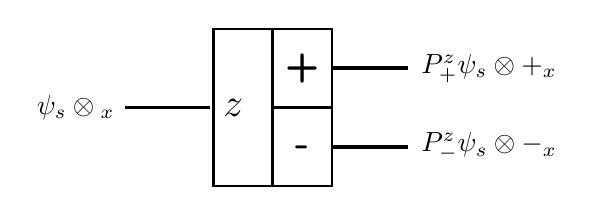
\begin{tikzpicture}[shorten >=1pt,auto, thick,
     square node/.style={rectangle, minimum height=2cm, minimum width=1.50cm, text width = 1.25cm, draw, font=\sffamily\Large\bfseries},
     port/.style={rectangle, draw,  minimum height=1cm, minimum width=0.75cm, font=\sffamily\Large\bfseries},
     wf/.style={rectangle, minimum height=1cm}]
    \apparatus{1}{2}{0}{$z$};

    \node(w0) at (-0.5,0) {$\ket{\psi_s} \otimes \ket{\varnothing_x}$};
    \node[wf] (w1) at (4.75, 0.5) {$P^z_+\ket{\psi_s} \otimes \ket{+_x}$};
    \node[wf] (w2) at (4.75, -0.5) {$P^z_-\ket{\psi_s} \otimes \ket{-_x}$};

    % \node(label1) at (0, -1.75) {$\bm{t_0}$};
    % \node(label2) at (6.25, -1.75) {$\bm{t_1}$};

    \draw[line width=0.5mm] (w0) -- (1);
    \draw[line width=0.5mm] (1+) -- (w1);
    \draw[line width=0.5mm] (1-) -- (w2);
\end{tikzpicture}

\caption[Insert an abbreviated caption here to show in the List of Figures]
{The Stern-Gerlach experiment as described by the von Neumann measurement scheme. Each measurement outcome corresponds to a term in the time-evolved state (TODO REF). Notice that the measurement interaction results in a branching structure, represented here as a tree graph with the apparatus as a node.}
\label{Figure:Measurement:DetectorStates}
\end{figure}

\section{Preferred Basis Problem}
TODO: discuss schmidt's theorem

\section{Inselection}

The von Neumann measurement scheme was originally written as entangling a microscopic system with a macroscopic apparatus \cite{von Neumann}. Yet, it is common that the position of the electron is used to represent that state of the apparatus. This is a useful and accurate abstraction, as the state of the apparatus for an ``up'' measurement must be correlated with with the ``up'' position state. However, this description is incomplete as it conflates the apparatus with the position system belonging to the electron. We now formalize the spin-position-apparatus interaction, similar to how the implied spin-position correlation in the projection postulate was formalized.

Newton's third law asserts that the force exerted on the electron by the apparatus magnet is paired with a force exerted on the magnet by the electron \cite{Newton}. This motivates the definition of apparatus states $\{\ket{+_a}, \ket{-_a}, \ket{\varnothing_a}\}$ representing the effect of positive, negative, and zero torques on the magnet, respectively. These apparatus states are classically distinguishable
\begin{align}
    \braket{i_a|j_a} = 0 \\
    &\forall i \neq j
\end{align}
and exhaustive. These states are somtimes called \textit{pointer states} in literature \cite{Zeh}, with $\ket{\varnothing_a}$ called the \textit{ready state}.

\subsection{Example 1}
Our system is now composed of spin, position, and apparatus systems $H = H_s \otimes H_x \otimes H_a$. We expect
\begin{align}
    \nonumber U(t_1, t_0): \\
    & \ket{\psi} = \left(\sum_{n} P^z_n\ket{\psi_s}\right) \otimes \ket{\varnothing_x} \otimes \ket{\varnothing_a} \mapsto \sum_{n}\left(P^z_n\ket{\psi_s} \otimes \ket{n_x} \otimes \ket{n_a} \right)
\end{align}
where $n = +, -$. This is accomplished by
\begin{align}
  U(t_1, t_0) &= P^z_+ \otimes \left(\: \ket{+_x}\bra{\varnothing_x} \: \bm{+} \: \ket{\varnothing_x}\bra{+_x} \: \bm{+} \: \ket{-_x}\bra{-_x} \: \right) \\ \nonumber
  &\phantom{{}=P^z_+} \otimes \left(\: \ket{+_a}\bra{\varnothing_a} \: \bm{+} \: \ket{\varnothing_a}\bra{+_a} \: \bm{+} \: \ket{-_a}\bra{-_a} \: \right)\\ \nonumber
  &+ P^z_- \otimes \left( \: \ket{-_x}\bra{\varnothing_x} \: \bm{+} \: \ket{\varnothing_x}\bra{-_x} \: \bm{+} \: \ket{+_x}\bra{+_x} \: \right) \\ \nonumber
 &\phantom{{}=P^z_-} \otimes \left(\: \ket{-_a}\bra{\varnothing_a} \: \bm{+} \: \ket{\varnothing_a}\bra{-_a} \: \bm{+} \: \ket{+_a}\bra{+_a} \: \right)
\end{align}

TODO: show PFBP is solved.

We could solve the preferred basis problem by including the environment rather than the apparatus. Such an approach is called superselection. However, the apparatus must exist by Newton's third law, and it solves the problem without reference to the environment. So, it seems reasonable that the configuration of the measurement fixes the basis (reflected in dynamics), as the basis we observe is a property of the apparatus. We will see that the role of the environment is to record the history TODO.

\begin{figure}
\centering\CaptionFontSize
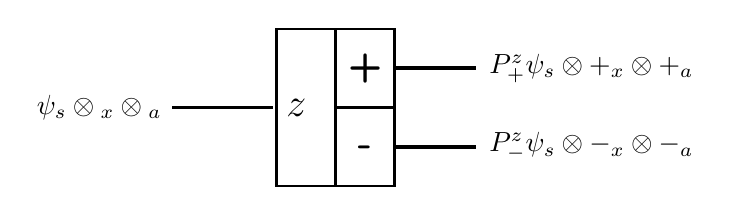
\begin{tikzpicture}[shorten >=1pt,auto, thick,
     square node/.style={rectangle, minimum height=2cm, minimum width=1.50cm, text width = 1.25cm, draw, font=\sffamily\Large\bfseries},
     port/.style={rectangle, draw,  minimum height=1cm, minimum width=0.75cm, font=\sffamily\Large\bfseries},
     wf/.style={rectangle, minimum height=1cm}]
    \apparatus{1}{2}{0}{$z$};

    \node(w0) at (-1,0) {$\ket{\psi_s} \otimes \ket{\varnothing_x} \otimes \ket{\varnothing_a}$};
    \node[wf] (w1) at (5.25, 0.5) {$P^z_+\ket{\psi_s} \otimes \ket{+_x} \otimes \ket{+_a}$};
    \node[wf] (w2) at (5.25, -0.5) {$P^z_-\ket{\psi_s} \otimes \ket{-_x} \otimes \ket{-_a}$};

    % \node(label1) at (0, -1.75) {$\bm{t_0}$};
    % \node(label2) at (6.25, -1.75) {$\bm{t_1}$};

    \draw[line width=0.5mm] (w0) -- (1);
    \draw[line width=0.5mm] (1+) -- (w1);
    \draw[line width=0.5mm] (1-) -- (w2);
\end{tikzpicture}
\caption[Insert an abbreviated caption here to show in the List of Figures]
{The most complete description of Experiment 1 presented, including position and apparatus degres of freedom. The seemingly redundant correlation of both position and apparatus states to spin states makes the abstraction of position states as apparatus states valid. However, formalizing the interaction with the apparatus provides a more complete description that resolves the preferred basis problem.}
\label{Figure:Measurement:DetectorStates}
\end{figure}

\section{Consecutive Measurements}
TODO: introduce assumptions of consecutive measurement.

The von Neumann measurement scheme can be applied succesively. Its operator is lengthy; in anticipation, we name the ``entanglement operator''
\begin{align}
  E^i_\pm &= \ket{\pm_i}\bra{\varnothing_i} \: \bm{+} \: \ket{\varnothing_i}\bra{\pm_i} \: \bm{+} \: \ket{\mp_i}\bra{\mp_i}
\end{align}
so that
\begin{align}
  U(t_1, t_0) &= P^z_+ \otimes E^x_+ \otimes E^a_+ \\ \nonumber
  &+ P^z_- \otimes E^x_- \otimes E^a_-
\end{align}

$E$ is Hermitian $\left(E^\dagger = E\right)$ and unitary $\left( E^\dagger E = I \right)$.

\subsection{Example 2}
Now that we have two apparatuses, the Hilbert space includes two pointer spaces: $\mathcal{H} = \mathcal{H}_s \otimes \mathcal{H}_x \otimes \mathcal{H}_{a_1} \otimes \mathcal{H}_{a_2}$. We also add two new coarse grained position states for the second apparatus. The position states are now $\{\ket{+_{x_1}}, \ket{-_{x_1}}, \ket{+_{x_2}}, \ket{-_{x_2}}, \ket{\varnothing_x}\}$, where $\ket{\varnothing_x}$ is any position not in either apparatus' spin-up or spin-down region. TODO: figure.

The dynamics are unchanged from TODO REF Example 1 for the first measurement, with the identity acting on the second apparatus to leave it unaffected:
\begin{align}
  U(t_1, t_0)_{a_1} &= P^z_+ \otimes E^{x_1}_+  \nonumber \otimes E^{a_1}_+ \otimes I_{a_2}\\ \nonumber
  &+ P^z_- \otimes E^{x_1}_-\otimes E^{a_1}_- \otimes I_{a_2}
\end{align}

Now we determine the dynamics for the second measurement. We expect the dynamics to do two things: revers the entanglements from the first measurement, and entangle the second apparatus with spin and position eigenstates. We return the first apparatus to the ready state, as it is no longer measuring the system and no torque is exerted on the magnet, and return position back to $\ket{\varnothing_x}$ as the electron leaves the analyzer. $U(t_1, t_0)^\dagger$ reverses the entanglement, but conveniently, $U(t_1, t_0)$ is Hermitian. So, the $a_1$ component of the unitary operator for the second measurement is the same as that of the first measurement:
\begin{align}
  U(t_2, t_1)_{a_1} &= U(t_1, t_0)
\end{align}

For the $a_2$ component, we want to entangle pointer states with position and spin states only when the first apparatus has measured spin-up. In the branch where spin-down has been measured, we use the identity operator $I = I_s \otimes I_x \otimes I_{a_1} \otimes I_{a_2}$ to represent the lack of a second measurement. In the branch where spin-up has been measured, we apply the measurement scheme again. The $a_2$ component of the unitary operator during second measurement is
\begin{align}
  U(t_2, t_1)_{a_2} &= P^x_+ P^z_+ \otimes E^{x_2}_+ \otimes I_{a_1} \otimes E^{a_2}_+ \\ \nonumber
  &+ P^x_- P^z_+ \otimes E^{x_2}_- \otimes I_{a_1} \otimes E^{a_2}_- \\ \nonumber
  &+ P^z_- \otimes{I_x} \otimes I_{a_1} \otimes I_{a_2}
\end{align}

So the complete unitary operator for the second measurement is
\begin{align}
  U(t_2, t_1) &= U(t_2, t_1)_{a_2} U(t_2, t_1)_{a_1} \\ \nonumber
  &= P^x_+ P^z_+ \otimes E^{x_2}_+  E^{x_1}_+ \otimes E^{a_1}_+ \otimes E^{a_2}_+ \\ \nonumber
  &+ P^x_- P^z_+ \otimes E^{x_2}_-  E^{x_1}_+ \otimes E^{a_1}_+ \otimes E^{a_2}_- \\ \nonumber
  &+ P^z_- \otimes E^{x_1}_- \otimes E^{a_1}_- \otimes I_{a_2}
\end{align}
and the final state is represented in Figure TODO REF.
% \begin{align}
%   U(t_2, t_1) &= U(t_2, t_1)_{a_1} U(t_2, t_1)_{a_2} \\ \nonumber
%   &= P^x_+ P^z_+ \otimes \left(\ket{+_{a_1}}\bra{\varnothing_{a_1}} \: \bm{+} \: \ket{\varnothing_{a_1}}\bra{+_{a_1}} \: \bm{+} \: \ket{-_{a_1}}\bra{-_{a_1}} \right) \\ \nonumber
%   & \phantom{{} = P^x_+ P^z_+} \otimes  \left(\ket{+_{a_2}}\bra{\varnothing_{a_2}} \: \bm{+} \: \ket{\varnothing_{a_2}}\bra{+_{a_2}} \: \bm{+} \: \ket{-_{a_2}}\bra{-_{a_2}} \right) \\ \nonumber
%   &+ P^x_- P^z_+ \otimes \left(\ket{+_{a_1}}\bra{\varnothing_{a_1}} \: \bm{+} \: \ket{\varnothing_{a_1}}\bra{+_{a_1}} \: \bm{+} \: \ket{-_{a_1}}\bra{-_{a_1}} \right) \\ \nonumber
%   & \phantom{{} = P^x_+ P^z_+} \otimes  \left(\ket{-_{a_2}}\bra{\varnothing_{a_2}} \: \bm{+} \: \ket{\varnothing_{a_2}}\bra{-_{a_2}} \: \bm{+} \: \ket{+_{a_2}}\bra{+_{a_2}} \right) \\ \nonumber
%   &+ P^z_- \otimes \left(\ket{-_{a_1}}\bra{\varnothing_{a_1}} \: \bm{+} \: \ket{\varnothing_{a_1}}\bra{-_{a_1}} \: \bm{+} \: \ket{+_{a_1}}\bra{+_{a_1}} \right) \\ \nonumber
%   & \phantom{{}={}P^z_+} \otimes I_{a_2}
% \end{align}

\begin{figure}
\centering\CaptionFontSize

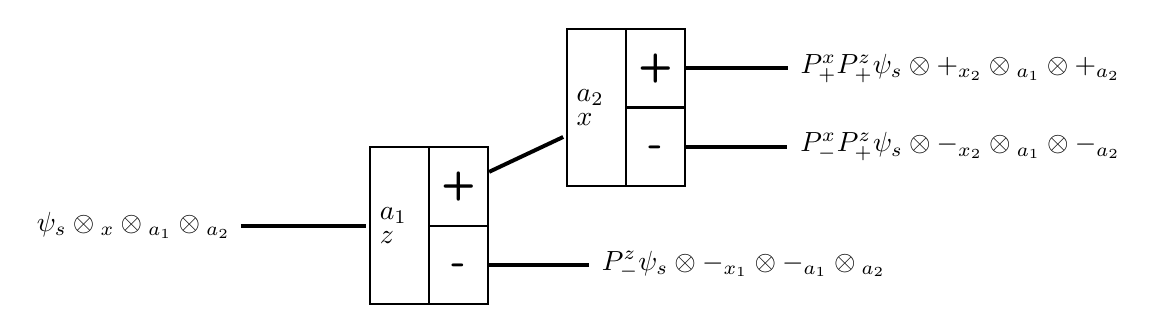
\begin{tikzpicture}[shorten >=1pt,auto, thick,
     square node/.style={rectangle, minimum height=2cm, minimum width=1.50cm, text width = 1.25cm, draw, font=\sffamily\Large\bfseries},
     port/.style={rectangle, draw,  minimum height=1cm, minimum width=0.75cm, font=\sffamily\Large\bfseries},
     wf/.style={rectangle, minimum height=1cm}]
    \apparatus{1}{4}{0}{${}^{a_1}_z$};
    \apparatus{2}{6.5}{1.5}{${}^{a_2}_x$};

    \node(w0) at (0.25,0) {$\ket{\psi_s} \otimes \ket{\varnothing_x} \otimes \ket{\varnothing_{a_1}} \otimes \ket{\varnothing_{a_2}} $};
    \node[wf] (w1) at (8, -.5) {$P^z_-\ket{\psi_s} \otimes \ket{-_{x_1}}  \otimes \ket{-_{a_1}} \otimes \ket{\varnothing_{a_2}}$};
    \node[wf] (w2) at (10.75, 1) {$P^x_-P^z_+\ket{\psi}_s \otimes \ket{-_{x_2}} \otimes \ket{\varnothing_{a_1}} \otimes \ket{-_{a_2}}$};
    \node[wf] (w3) at (10.75, 2) {$P^x_+ P^z_+\ket{\psi_s} \otimes \ket{+_{x_2}} \otimes \ket{\varnothing_{a_1}} \otimes \ket{+_{a_2}}$};

    % \node(label0) at (0, -1.75) {$\bm{t_0}$};
    % \node(label1) at (4.75, -1.75) {$\bm{t_1}$};
    % \node(label2) at (7.25, -1.75) {$\bm{t_2}$};
    % \node(label3) at (9.75, -1.75) {$\bm{t_3}$};
    % \node(bw1) at (-1.75, 1.75) {$P^z_+\ket{\psi}^s \otimes \ket{+}^{D_1}_z \otimes \ket{\varnothing}^{D_2}_x $};

    \draw[line width=0.5mm] (w0) -- (1);
    \draw[line width=0.5mm] (1+) -- (2);
    \draw[line width=0.5mm] (1-) --  (w1);
    \draw[line width=0.5mm] (2+) -- (w3);
    \draw[line width=0.5mm] (2-) -- (w2);


\end{tikzpicture}

\caption[Insert an abbreviated caption here to show in the List of Figures]
{TODO: caption}
\label{Figure:Measurement:labelthis2}
\end{figure}

% \subsection{Example 3}
%
%
% \begin{figure}
% \centering\CaptionFontSize
% % \begin{tikzpicture}[shorten >=1pt,auto, thick,
% %      square node/.style={rectangle, minimum height=2cm, minimum width=1.50cm, text width = 1.25cm, draw, font=\sffamily\Large\bfseries},
% %      port/.style={rectangle, draw,  minimum height=1cm, minimum width=0.75cm, font=\sffamily\Large\bfseries},
% %      wf/.style={rectangle, minimum height=1cm}]
% %     \apparatus{1}{-4}{0}{$Z$};
% %     \apparatus{2}{2}{1.5}{$X$};
% %     \apparatus{3}{2}{-1.5}{$X$};
% %
% %     \node(w0) at (-8,0) {$\ket{\psi}^s \otimes \ket{\varnothing}^{D_1}_z \otimes \ket{\varnothing}^{D_2}_x \otimes \ket{\varnothing}^{D_3}_x$};
% %     \node[wf] (w1) at (6, 2) {$P^x_+ P^z_+\ket{\psi}^s \otimes \ket{\varnothing}^{D_1}_z \otimes \ket{+}^{D_2}_x \otimes \ket{\varnothing}^{D_3}_x$};
% %     \node[wf] (w2) at (8.25, 1) {${P^x}_-{P^z}_-\ket{\psi}_s \otimes \ket{\mathcal{X}_-}_z$};
% %     \node[wf] (w3) at (8.25, -1) {${P^z}_+\ket{\psi}_s \otimes \ket{\mathcal{X}_+}_z$};
% %     \node[wf] (w4) at (8.25, -2) {${P^z}_-\ket{\psi}_s \otimes \ket{\mathcal{X}_-}_z$};
% %
% %     % \node(label1) at (0, -1.75) {$\bm{t_0}$};
% %     % \node(label2) at (6.25, -1.75) {$\bm{t_1}$};
% %     \node(bw1) at (-1.75, 1.75) {$P^z_+\ket{\psi}^s \otimes \ket{+}^{D_1}_z \otimes \ket{\varnothing}^{D_2}_x \otimes \ket{\varnothing}^{D_3}_x$};
% %
% %     \node(bw2) at (-1.75, -1.75) {$P^z_-\ket{\psi}^s \otimes \ket{-}^{D_1}_z \otimes \ket{\varnothing}^{D_2}_x \otimes \ket{\varnothing}^{D_3}_x$};
% %
% %     \draw[line width=0.5mm] (w0) -- (1);
% %     \draw[line width=0.5mm] (1+) -- (2);
% %     \draw[line width=0.5mm] (1-) --  (3);
% %     \draw[line width=0.5mm] (2+) -- (w1);
% %     \draw[line width=0.5mm] (2-) -- (w2);
% %     \draw[line width=0.5mm] (3+) -- (w3);
% %     \draw[line width=0.5mm] (3-) -- (w4);
% % \end{tikzpicture}
% \begin{adjustbox}{width=\textwidth}
% \begin{tikzpicture}[shorten >=1pt,auto, thick,
%      square node/.style={rectangle, minimum height=2cm, minimum width=1.50cm, text width = 1.25cm, draw, font=\sffamily\Large\bfseries},
%      port/.style={rectangle, draw,  minimum height=1cm, minimum width=0.75cm, font=\sffamily\Large\bfseries},
%      wf/.style={rectangle, minimum height=1cm}]
%     \apparatus{1}{4}{0}{${}^{D_1}_z$};
%     \apparatus{2}{6.5}{1.5}{${}^{D_2}_x$};
%     \apparatus{3}{9}{3}{${}^{D_3}_z$};
%
%     \node(w0) at (0,0) {$\ket{\psi_s} \otimes \ket{\varnothing_{D_1}} \otimes \ket{\varnothing_{D_2}} \otimes \ket{\varnothing_{D_3}}$};
%     \node[wf] (w1) at (8, -.5) {$ P^z_-\ket{\psi_s} \otimes \ket{-_{D_1}} \otimes \ket{\varnothing_{D_2}} \otimes \ket{\varnothing_{D_3}} $};
%     \node[wf] (w2) at (10.75, 1) {$P^x_-P^z_+\ket{\psi}_s \otimes \ket{\varnothing_{D_1}} \otimes \ket{-_{D_2}} \otimes \ket{\varnothing_{D_3}} $};
%     \node[wf] (w3) at (13.5, 3.5) {$P^z_+ P^x_+ P^z_+\ket{\psi_s} \otimes \ket{\varnothing_{D_1}} \otimes \ket{\varnothing_{D_2}} \otimes \ket{+_{D_3}}$};
%     \node[wf] (w4) at (13.5, 2.5) {$P^z_- P^x_+ P^z_+ \ket{\psi_s} \otimes \ket{\varnothing_{D_1}} \otimes \ket{\varnothing_{D_2}} \otimes \ket{-_{D_3}} $};
%
%     % \node(label0) at (0, -1.75) {$\bm{t_0}$};
%     % \node(label1) at (4.75, -1.75) {$\bm{t_1}$};
%     % \node(label2) at (7.25, -1.75) {$\bm{t_2}$};
%     % \node(label3) at (9.75, -1.75) {$\bm{t_3}$};
%     % \node(bw1) at (-1.75, 1.75) {$P^z_+\ket{\psi}^s \otimes \ket{+}^{D_1}_z \otimes \ket{\varnothing}^{D_2}_x $};
%
%     \draw[line width=0.5mm] (w0) -- (1);
%     \draw[line width=0.5mm] (1+) -- (2);
%     \draw[line width=0.5mm] (1-) --  (w1);
%     \draw[line width=0.5mm] (2+) -- (3);
%     \draw[line width=0.5mm] (2-) -- (w2);
%     \draw[line width=0.5mm] (3+) -- (w3);
%     \draw[line width=0.5mm] (3-) -- (w4);
%
% \end{tikzpicture}
% \end{adjustbox}
%
% \caption[Insert an abbreviated caption here to show in the List of Figures]
% {The Stern-Gerlach experiment as described by the von Neumann measurement scheme. Each measurement outcome corresponds to a term in the time-evolved state (Eq 4.4). Notice that the measurement interaction results in a branching structure, which is represented here visually with a tree graph. }
% \label{Figure:Measurement:labelthis}
% \end{figure}

% There is no one ``measurement problem'' of standard quantum mechanics,
%
% By discarding the projection postulate, no notion of an undefined ``interaction with a classical apparatus'' is required to describe how states evolve when their properties are recorded. The various paradoxes and interpretational issues associated with state collapse are entirely circumvented.
%
